\section{LENA Performance and Energy Usage}

As described in Section \ref{sec:perf-focus}, a major goal of our
project was to acheive frame rates of at least 10 frames per second for
unprocessed video. This goal attends to our group's assignment of
focusing on performance.

Here we present results from running different image processing programs
on the system. For each program a frame rate is listed. This is the
maximum frame rate at which the program could be run without generating
artifacts on the screen. We also list power consumption for
each of the programs. These measurements were made using an ammeter
across the headers connecting the power planes to 12 V.

\subsection{Test programs}

Here are the numbered test programs used to generate the results:

\begin{description}
    \item[Program 1] \hfill \\
        Show unprocessed video on the screen using only the control
        core. The control core's task is to continually copy the
        incoming image data into the screen buffer.
    \item[Program 2] \hfill \\
        Show video with inverted colors, using only the control core.
        The control core operates as in program 1, but it subtracts the
        pixel values from 255 before copying them to the screen buffer.
    \item[Program 3] \hfill \\
        Show unprocessed video using the SIMD nodes. All of the pixels
        in a video frame are sent through the SIMD array before being
        copied to the screen by the control core.
    \item[Program 4] \hfill \\
        Show inverted video using the SIMD nodes. The SIMD cores operate
        as in program 3, but they invert the pixel colors before passing
        the pixels back out to data RAM.
    \item[Program 5] \hfill \\
        Show video processed by a 3x3 edge detection filter on the SIMD
        nodes.
\end{description}

\subsection{Results}

The test results are listed in Table \ref{tab:lena-benchmark-table} and
plotted in Figure \ref{fig:lena-benchmark-plot}. 

\begin{table}[h!]
\centering
\begin{tabular}{c|r|rrr|r} \toprule
	\multirow{2}{*}{\textbf{Program}} &
        \multirow{2}{*}{\textbf{Frame rate}} &
        \multicolumn{3}{c|}{\textbf{Current through power planes}} &
        \multirow{2}{*}{\textbf{Power}} \\
        & &
        \textbf{3.3 V} &
        \textbf{2.5 V} &
        \textbf{1.2 V} & \\
	\midrule
	\emph{Idle} & - & 347 mA & 44 mA & 77 mA & 5.6 W \\
	1 & 21 fps & 375 mA & 37 mA & 69 mA & 5.8 W \\
        2 & 18 fps & 375 mA & 37 mA & 71 mA & 5.8 W \\
        3 & 13 fps & 370 mA & 37 mA & 65 mA & 5.7 W \\
        4 & 13 fps & 375 mA & 37 mA & 67 mA & 5.7 W \\
        5 & 13 fps & 363 mA & 37 mA & 75 mA & 5.7 W \\ \bottomrule
\end{tabular}
\caption[LENA results]{LENA performance and power results.}
\label{tab:lena-benchmark-table}
\end{table}

\begin{figure}[h!]
\centering
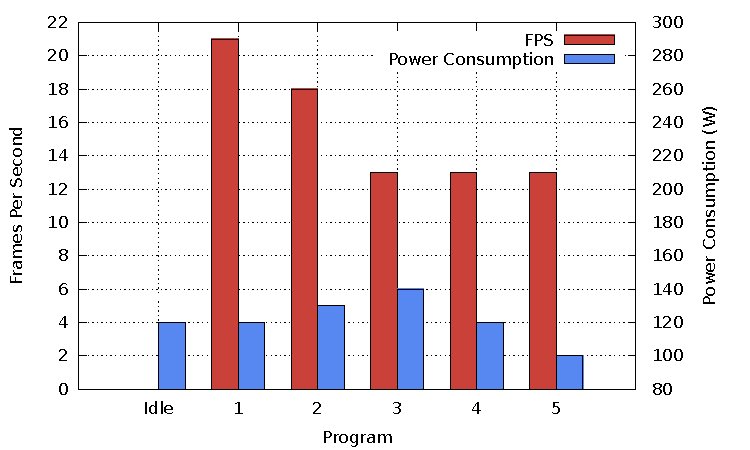
\includegraphics[width=\textwidth]{fig/res/lena-benchmark-plot.pdf}
\caption[LENA results]{The LENA results from Table
\ref{tab:lena-benchmark-table}.}
\label{fig:lena-benchmark-plot}
\end{figure}


The system performance behaved as expected. The fastest program was
program 1, which simply performs a copy iteration from data RAM to video
RAM. This is a step the other programs have to perform as well. Program
2 is slightly slower than program 1, which probably is due to the extra
subtraction in the inner loop of the program.

Programs 3, 4 and 5 are slower than the previous two programs. The
copying of data into and out of the SIMD array entails a certain
overhead that cannot be avoided. However, the increase in complexity in
the programs from 3 to 5, does not result in a decrease in their
performance. This is because all of the three programs are limited by
the DMA speed, not the computational speed. Data transfer is the
bottleneck in all of the three programs.

The power consumption stays relatively stable throughout the tests. This
was to be expected, as no power management features have been
implemented in the system.
